
\section{Execution Environment}\label{sec:execution_environment}

Performing a software build requires the build activities to execute in the
proper execution environment.  The execution environment is often configured
as a "build box" or a container defined as the execution environment in
a pipeline build stage.  The build environment will typically have all the
tools and configuration required to perform a software build intended 
to yield an package 
containing executable software.  As part of the build, the resolution of 
dependencies is typically part of one or more build steps.  This is often 
required for the software to compile and/or to produce
a distributable build output.\footnote{Not all languages require a compile
or to have dependencies available for the distributable packaging.
The hypothetical scenario discussed is that the dependencies need to be
available at some point during software development if they are 
used by the software at runtime.}

Obtaining an accurate dependency resolution requires the dependency tree to be
resolved in the correct execution environment.  This applies to not only the
availability of the tools and configuration required to resolve 
the dependencies, but also to
the network accessibility where the dependency resolution is executed.  It
frequently the case that dependencies are obtained by network services
accessible only when originating a request from an organization's network. 
In cases such as the one illustrated in Figure \ref{fig:dependency_tree},
the vulnerable transitive dependency of an internally developed package may
not be detected in some scenarios.



\subsubsection{Execution Environment Happy Path}\label{sssec:happy_path}

Figure \ref{fig:dependency_resolution_happy_path} illustrates the concept
of a basic dependency resolution happy path.  In the diagram, the supply chain
scan is added to an existing pipeline to perform dependency resolution
and obtain the dependency tree required for the scan.  The dependency tree is
then sent to the scanning service where the tree is assessed for 
vulnerable packages.

The reason this works is that the dependency resolution is executed inside of
the very same environment used to build the software.  Not only is the correct 
tooling available and properly configured, it is run with the same network
accessibility that allows any private packages to be resolved during the build.

A build environment may serve one or more projects that have the same tooling,
configuration, and network accessibility requirements.  As part of configuring
the ability to build the software, the correct environment for the project
is often defined as part of the pipeline definition.  

As an example, refer to the 
\hyperref[listing:ado_pipeline]{\texttt{Azure Devops Pipeline Example}} listing.
It can be observed in the example pipeline definition that the \texttt{container} 
or \texttt{pool} directives can be used to give the pipeline stage execution an affinity 
for a specific build box or container. When the dependency resolution and supply chain scan
is executed, the execution is in an environment that contains all the tools
needed for a successful scan.



\begin{figure}[h]
    \caption{Dependency Resolution Execution Happy Path}
    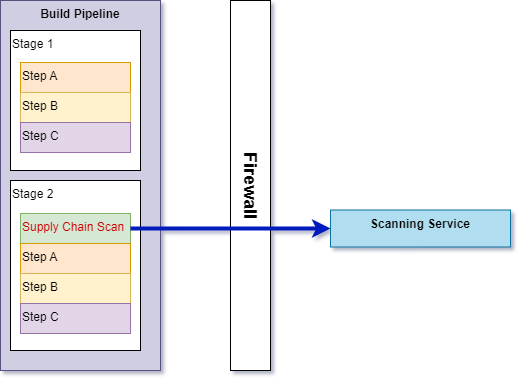
\includegraphics[width=\textwidth]{graphics/dependency_resolution_happy_path.png}
    \label{fig:dependency_resolution_happy_path}
\end{figure}



\label{listing:ado_pipeline}
\begin{code}{Azure Devops Pipeline Example}{}{}
trigger:
    - master

pool:
    vmImage: ubuntu-latest

jobs:
    - job: SCAResolver
        pool:
            vmImage: ubuntu-latest

        container: 
            image: cxnleach/scaresolver-general-build-ado:latest

        steps:
            - script: /sandbox/resolver/ScaResolver -h
\end{code}




\subsubsection{Generic Execution Environment}\label{sssec:generic_environment}

Figure \ref{fig:dependency_resolution_generic_env} depicts a build pipeline that
submits the code or build definition files to a remote service for dependency
resolution and supply chain scanning.  It is very similar to the scenario
described previously in \hyperref[sssec:happy_path]{\textit{Execution Environment Happy Path}}
with the difference being that the dependency resolution is executing in
an execution environment provided by the remote system.  The remote system may not have the
ability to define a specific execution environment for dependency resolution as can
be done within a pipeline definition.

In this scenario, the generic build environment must have properly installed and configured
all tools required to successfully perform a dependency resolution.  In some cases, 
the tooling installation and configuration requirements is simple and this will work.  There
are other cases where this may not be so simple:

\begin{itemize}
    \item The dependency resolution requires older or newer versions of the build tools.
    \item The build tools are not compatible with the remote platform's build environment.
    \item Internally built or third-party licensed tools are required.
    \item Specific tooling configurations are required to perform the build.
\end{itemize}

If the tooling and configuration is not correctly defined in the generic environment,
the dependency resolution may not accurately produce a dependency tree.

\begin{figure}[h]
    \caption{Dependency Resolution Generic Execution Environment}
    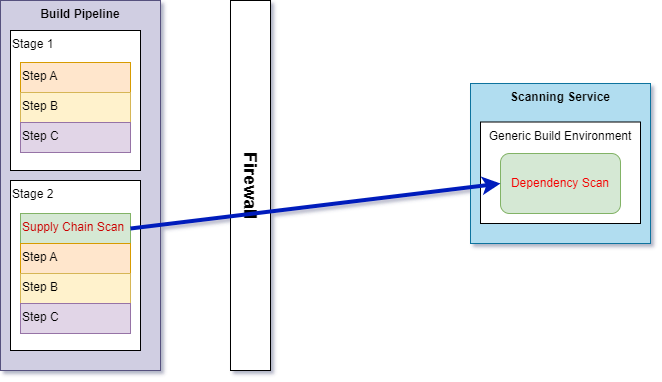
\includegraphics[width=\textwidth]{graphics/dependency_resolution_generic_env.png}
    \label{fig:dependency_resolution_generic_env}
\end{figure}



\subsubsection{Remote Execution Environment}

A remote execution environment is a variation of the 
\hyperref[sssec:generic_environment]{\texttt{Generic Execution Environment}}.  In this
environment, the build environment can be generic or it can have the correct tooling
and configuration necessary to produce a build.  The challenge here is that the network
paths available to the remote execution environment may not allow for an accurate
dependency tree to be generated.

Figure \ref{fig:dependency_resolution} shows the diagram of the network connections
used during the dependency resolution.  The remote environment will generally have
no issues accessing public package repositories to resolve open source direct and transitive
dependencies.  The red line shows an attempted network connection to a package
repository that may be accessible only from within the corporate network.  When the
supply chain scan submits the scan so that dependency resolution occurs in the
remote environment, the network connection may not be available.  

If \texttt{Step A} of the pipeline's \texttt{Stage 2} is executed after the supply chain
scan, it is performed inside the corporate network.  The green line indicates that it can 
reach the internal package repository.  The internal package repository can be reached
since the execution of \texttt{Step A} is performed on the corporate network.

\begin{figure}[h]
    \caption{Dependency Resolution Remote Execution Environment}
    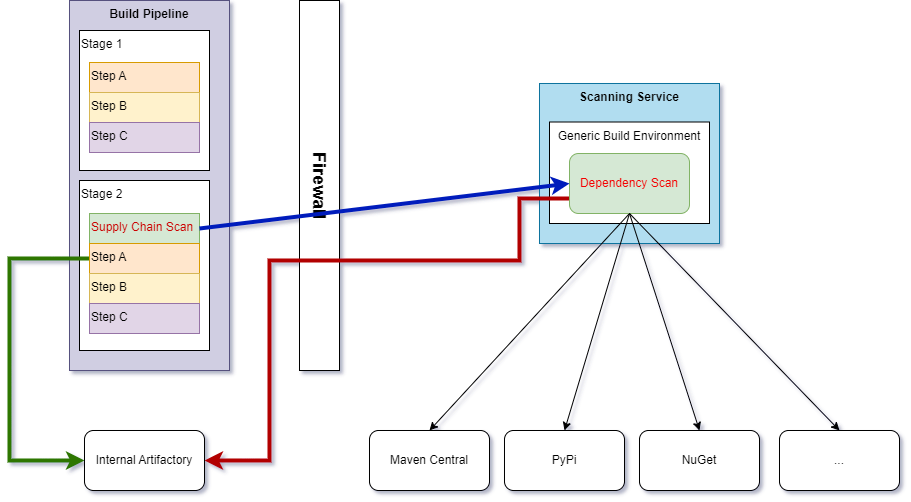
\includegraphics[width=\textwidth]{graphics/dependency_resolution.png}
    \label{fig:dependency_resolution}
\end{figure}

